\section{Triggers definition}

The typical syntax of a trigger is as follows:
\begin{lstlisting}[style=SQL]
CREATE TRIGGER <TriggerName>
{BEFORE|AFTER}
{INSERT|DELETE|UPDATE [OF <ColumnName>]} ON <TableName>
REFERENCING { 
                [OLD TABLE [AS] <OldTableAlias>]
                [NEW TABLE [AS] <NewTableAlias>] |
                [OLD [ROW] [AS] <OldTupleName>]
                [NEW [ROW] [AS] <NewTupleName>]
}
[FOR EACH {ROW|STATEMENT}]
[WHEN <Condition>]
<SQLProceduralStatement> 
\end{lstlisting}

\paragraph*{Modes}
Triggers can be executed in different modes, including:
\begin{itemize}
    \item \texttt{BEFORE}: in this mode, the trigger's action occurs before any changes to the database's status, but only if the specified condition is met.
        It is primarily used for validating modifications before they are applied, potentially allowing for conditional effects.
        A significant constraint is that "before" triggers cannot directly update the database. 
        However, they can impact transition variables at a row-level granularity, often implemented as: 
        \begin{lstlisting}[style=SQL]
SET NEW.t = <expression>
        \end{lstlisting}
    \item \texttt{AFTER}: this mode involves executing the trigger's action after the database has undergone modifications, contingent upon the satisfaction of the specified condition.
        It is the most commonly used mode and is well-suited for a wide range of applications.
\end{itemize}

\paragraph*{Granularity}
Triggers can function at various levels of granularity:
\begin{itemize}
    \item \textit{Row-level granularity}: tn this approach, the trigger is evaluated and potentially executed separately for each tuple affected by the triggering statement. 
        Writing triggers at the row-level is more straightforward but may be less efficient.
    \item \textit{Statement-level granularity}: triggers are assessed and potentially executed only once for each activating statement, regardless of the number of tuples impacted in the target table. 
        This occurs even if no tuple is affected. 
        This mode aligns more closely with the traditional SQL statement approach, which is typically set-oriented.
\end{itemize}
\begin{definition}[\textit{Transition variables}]
    In the context of triggers, transition variables are special variables that indicate the state of a modification, both \texttt{BEFORE} and \texttt{AFTER}. 
\end{definition}
The syntax depends on the level of granularity: 
\begin{itemize}
    \item Row-level: in this case, the variables old and new are used, where old represents the value before the modification of the specific row (tuple) being considered, and new represents the value after the modification.
    \item Statement-level: for this granularity, table variables are employed.
     These include old table and new table, with old table containing the old values of all affected rows and new table containing the new values of those rows.
\end{itemize}
It's important to note that, in specific cases, these variables may be undefined. 
In triggers with an event of \texttt{INSERT}, the variables old and old table are undefined, while in triggers with an event of \texttt{DELETE}, the variables new and new table are undefined.  
\begin{example}
    Table T2 serves as a replica of table T1. 
    Whenever an update is made to T1, this modification is automatically replicated in T2. 
    This replication process is accomplished using triggers.
    The insertion of a new tuple is done with the following trigger: 
    \begin{lstlisting}[style=SQL]
CREATE TRIGGER REPLIC_INS
AFTER INSERT ON T1
FOR EACH ROW
INSERT INTO T2 VALUES (NEW.ID, NEW.VALUE);
    \end{lstlisting}
    The deletion of a tuple is done with the following trigger: 
    \begin{lstlisting}[style=SQL]
CREATE TRIGGER REPLIC_DEL
AFTER DELETE ON T1
FOR EACH ROW
DELETE FROM T2 WHERE T2.ID = OLD.ID;
    \end{lstlisting}
    The update of only the value a tuple is done with the following trigger: 
    \begin{lstlisting}[style=SQL]
CREATE TRIGGER REPLIC_UPD
AFTER UPDATE OF VALUE ON T1
WHEN NEW.ID = OLD.ID
FOR EACH ROW
UPDATE T2 SET T2.VALUE = NEW.VALUE
WHERE T2.ID = OLD.ID;
    \end{lstlisting}
    The previously mentioned trigger will not activate when the ID of a tuple is modified. 
    Nonetheless, for a comprehensive and robust implementation, this scenario must also be taken into account.

    If we want to replicate the rows only for the tuples whose value is $\geq$ 10, we will have the following triggers: 
    \begin{lstlisting}[style=SQL]
-- Insertion
CREATE TRIGGER CON_REPL_INS
AFTER INSERT ON T1
FOR EACH ROW
WHEN (new.VALUE >= 10)
INSERT INTO T2 VALUES (new.ID, new.VALUE);
-- Deletion
CREATE TRIGGER Cond_REPL_DEL
AFTER DELETE ON T1
FOR EACH ROW
WHEN (old.VALUE >= 10)
DELETE FROM T2 WHERE T2.ID = old.ID;
    \end{lstlisting}
\end{example}

\paragraph*{Execution order}
When multiple triggers are linked to a common event, SQL:1999 dictates the sequence in which they execute: 
\begin{enumerate}
    \item \texttt{BEFORE} statement level triggers. 
    \item \texttt{BEFORE} row level triggers. 
    \item Modification is applied, and integrity constraints are checked.
    \item \texttt{AFTER} row level triggers. 
    \item \texttt{AFTER} statement level triggers.
\end{enumerate}
However, if there are multiple triggers within the same category, the order of execution is contingent upon the specific system's implementation.

\paragraph*{Cascading}
The action of a trigger can lead to the activation of another trigger, a phenomenon known as cascading or nesting.
Recursive cascading occurs when a statement, S, executed on table T initiates a sequence of triggers that generates the same event, S, on table T, often referred to as looping.
It is important to ensure that recursive cascading does not. produce undesired effects. 
\begin{definition}[\textit{Termination}]
    In the context of triggers, the concept of termination ensures that, regardless of the initial state and any sequence of modifications, there is always a definitive final state, thereby preventing the possibility of infinite activation cycles.
\end{definition}
The simplest check exploits the triggering graph, that consists of a node $i$ for each trigger $T_i$, and an arc from a node $i$ to a node $j$ if the execution of trigger $T_i$'s action may activate trigger $T_j$.
The graph is created through a straightforward syntactic analysis. 
If it is acyclic, the system will definitely terminate. 
However, in the presence of cycles, triggers may or may not terminate. 
It's important to emphasize that acyclicity is adequate for ensuring termination but not a mandatory requirement.
\begin{example}
    Consider the following triggers:
    \begin{lstlisting}[style=SQL]
-- T1
CREATE TRIGGER AdjustContributions
AFTER UPDATE OF Salary ON Employee
REFERENCING NEW TABLE AS NewEmp
FOR EACH STATEMENT
UPDATE Employee
SET Contribution = Salary * 0.8
WHERE RegNum IN (SELECT RegNum FROM NewEmp)
-- T2
CREATE TRIGGER CheckOverallBudgetThreshold
AFTER UPDATE ON Employee
WHEN (SELECT sum(Salary+Contribution) FROM Employee) > 50000
UPDATE Employee
SET Salary = 0.9 * Salary; 
    \end{lstlisting}
    The triggering graph associated with these triggers is illustrated below:
    \begin{figure}[H]
        \centering
        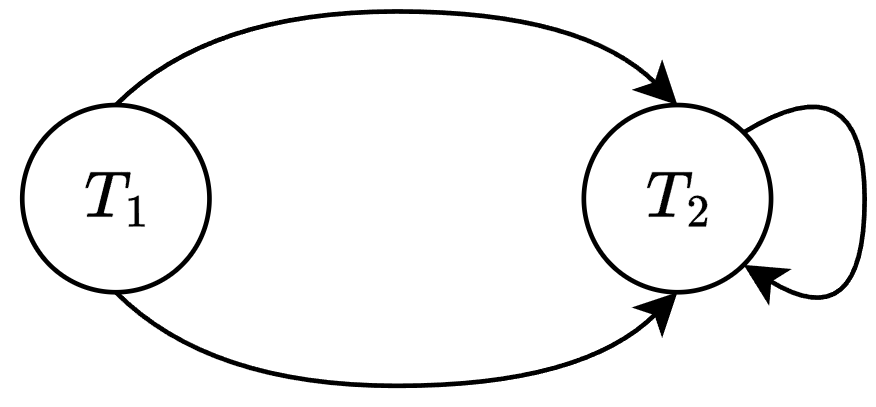
\includegraphics[width=0.25\linewidth]{images/trig.png}
    \end{figure}
    In this triggering graph, there are two cycles, but it's important to note that the system still terminates.
\end{example}